\documentclass[Analysis-3.tex]{subfiles}

\begin{document}
\chapter*{Lecture 19} %Set chapter name
\addcontentsline{toc}{chapter}{Lecture 19} %Set chapter title
\setcounter{chapter}{19} %Set chapter counter
\setcounter{section}{0}

\section{Integration over Bounded Domain}

Now that we know how to do integration over boxes, in this lecture we will discuss about how to integrate a bounded function over an arbitrary bounded set.

\

Let $\Omega \subseteq \R^n$, and $f \in \mathscr{B}(\Omega)$ and $\Omega$ bounded, then there exists $B^n \supseteq \Omega$ where $B^n = \prod_{i=1}^n [a_i, b_i]$.

\begin{Def}{}{}
    Given $\Omega$ bounded, let $B^n \supseteq \Omega$. For $f \in \mathscr{B}(\Omega)$, define
    \[
        \tilde{f}_{B^n}(x) = \begin{cases}
            f(x) & \mbox{ if } x \in \Omega               \\
            0    & \mbox{ if } x \in B^n \setminus \Omega
        \end{cases}
    \]
\end{Def}

An immediate question that arises now is: If $B^n \supseteq \Omega$ and $\hat{B^n} \supseteq \Omega$ then will it be true that
\begin{enumerate}
    \item[(1)] $\tilde{f}_{B^n} \in \mathscr{R}(B^n)$
    \item[(2)] And if $(1)$ holds, is it necessarily true that $\displaystyle{\int_{B^n} \tilde{f}_{B^n} = \int_{\hat{B^n}} \tilde{f}_{\hat{B^n}}}$.
\end{enumerate}
It is in fact true that $(1) \implies (2)$, but we won't cover the proof here.

\

\begin{Def}{}{}
    Let $f \in \mathscr{B}(\Omega)$. We say that $f \in \mathscr{R}(\Omega)$ if $\int_{B^n} \tilde{f}_{B^n}$ exists for some $B^n \supseteq \Omega$, and in this case we define
    \[
        \int_{\Omega} f := \int_{B^n} \tilde{f}_{B^n}
    \]
\end{Def}

\begin{Def}{Content Zero Sets}{}
    Let $S \subseteq \R^n$, we say that $S$ is of content zero if for all $\varepsilon > 0$, there exists boxes $\{ B_j^n \}_{j=1}^p$ (for some $p \in \N$) such that
    \[
        S \subseteq \bigcup_{j=1}^p B_j^n \quad \mbox{ and } \quad \sum_{j=1}^n \mathcal{V}(B^n_j) < \varepsilon
    \]
\end{Def}

For example a line segment in $\R^n$ is of content zero, provided $n > 1$. We then have the following theorems:

\begin{Thm}{}{}\label{thm1:19}
    \begin{enumerate}
        \item Let $f \in \mathscr{B}(B^n)$ and let $\mathcal{D} = \{ x \in B^n \mid f \mbox{ is not continuous at } x \}$ be the set of discontinuities of $f$, if $\mathcal{D}$ is of content zero, then $f \in \mathscr{R}(B^n)$.

        \item If $S$ is a content zero set then $\mathrm{int}\,(S) = \emptyset$.

        \item Let $\Omega \subseteq \R^n$ and $\mathcal{O}_n \subseteq \Omega$ is bounded. Let $f \in \mathscr{B}(\Omega)$ and $f\vert_{\mathcal{O}_n} \in \mathscr{C}(\mathcal{O}_n)$, if $\bar{\Omega}\setminus \mathcal{O}_n$ is content zero then $f \in \mathscr{R}(\Omega)$ and
              \[
                  \int_{\Omega} f = \int_{\mathcal{O}_n} f
              \]
    \end{enumerate}
\end{Thm}
Particularly part $(1)$ and $(3)$ of Theorem $\ref{thm1:19}$ are very important.

\

Now that we know how to integrate on arbitrary domains, the next question that comes to our mind is, does there exists a Fubini's theorem for integration over arbitrary sets? Before that we define elementary regions.

\section{Two Elementary Regions}

\begin{Def}{Elementary Regions}{}
    A set $\Omega \subseteq \R^2$ is $y$-simple/type I if there exists functions $\varphi_1, \varphi_2 \in \mathscr{B}([a,b])$ such that
    \[
        \Omega = \{ (x,y) \mid x \in [a,b], \, y \in [\varphi_1(x), \varphi_2(x)] \}
    \]
    Similarly a set $\Omega \subseteq \R^2$ is $x$-simple/type II if there exists functions $\psi_1, \psi_2 \in \mathscr{B}([c,d])$ such that
    \[
        \Omega = \{ (x,y) \mid y \in [c,d], \, x \in [ \psi_1(x), \psi_2(x) ] \}
    \]
\end{Def}

\begin{figure}[H]
    \centering
    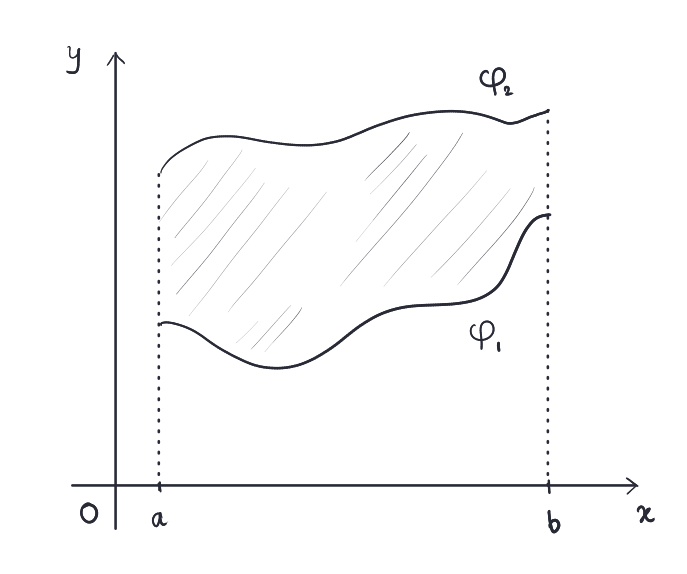
\includegraphics[width=0.5\textwidth]{../figures/ysimpleRegion.png}
    \caption{Example of a $y$-simple region.}
\end{figure}

\

% \textit{Examples (of elementary regions).} 
\begin{Eg}{Examples of elementary regions}{}
    The region $H$ given by
    \[
        H = \{ (x,y) \mid 0 \leq x \leq 1, \mbox{ and } x^2 \leq y \leq x \}
    \]
    is a $y$-simple region. (see figure $\ref{fig1:19}$)
    \begin{figure}[H]
        \centering
        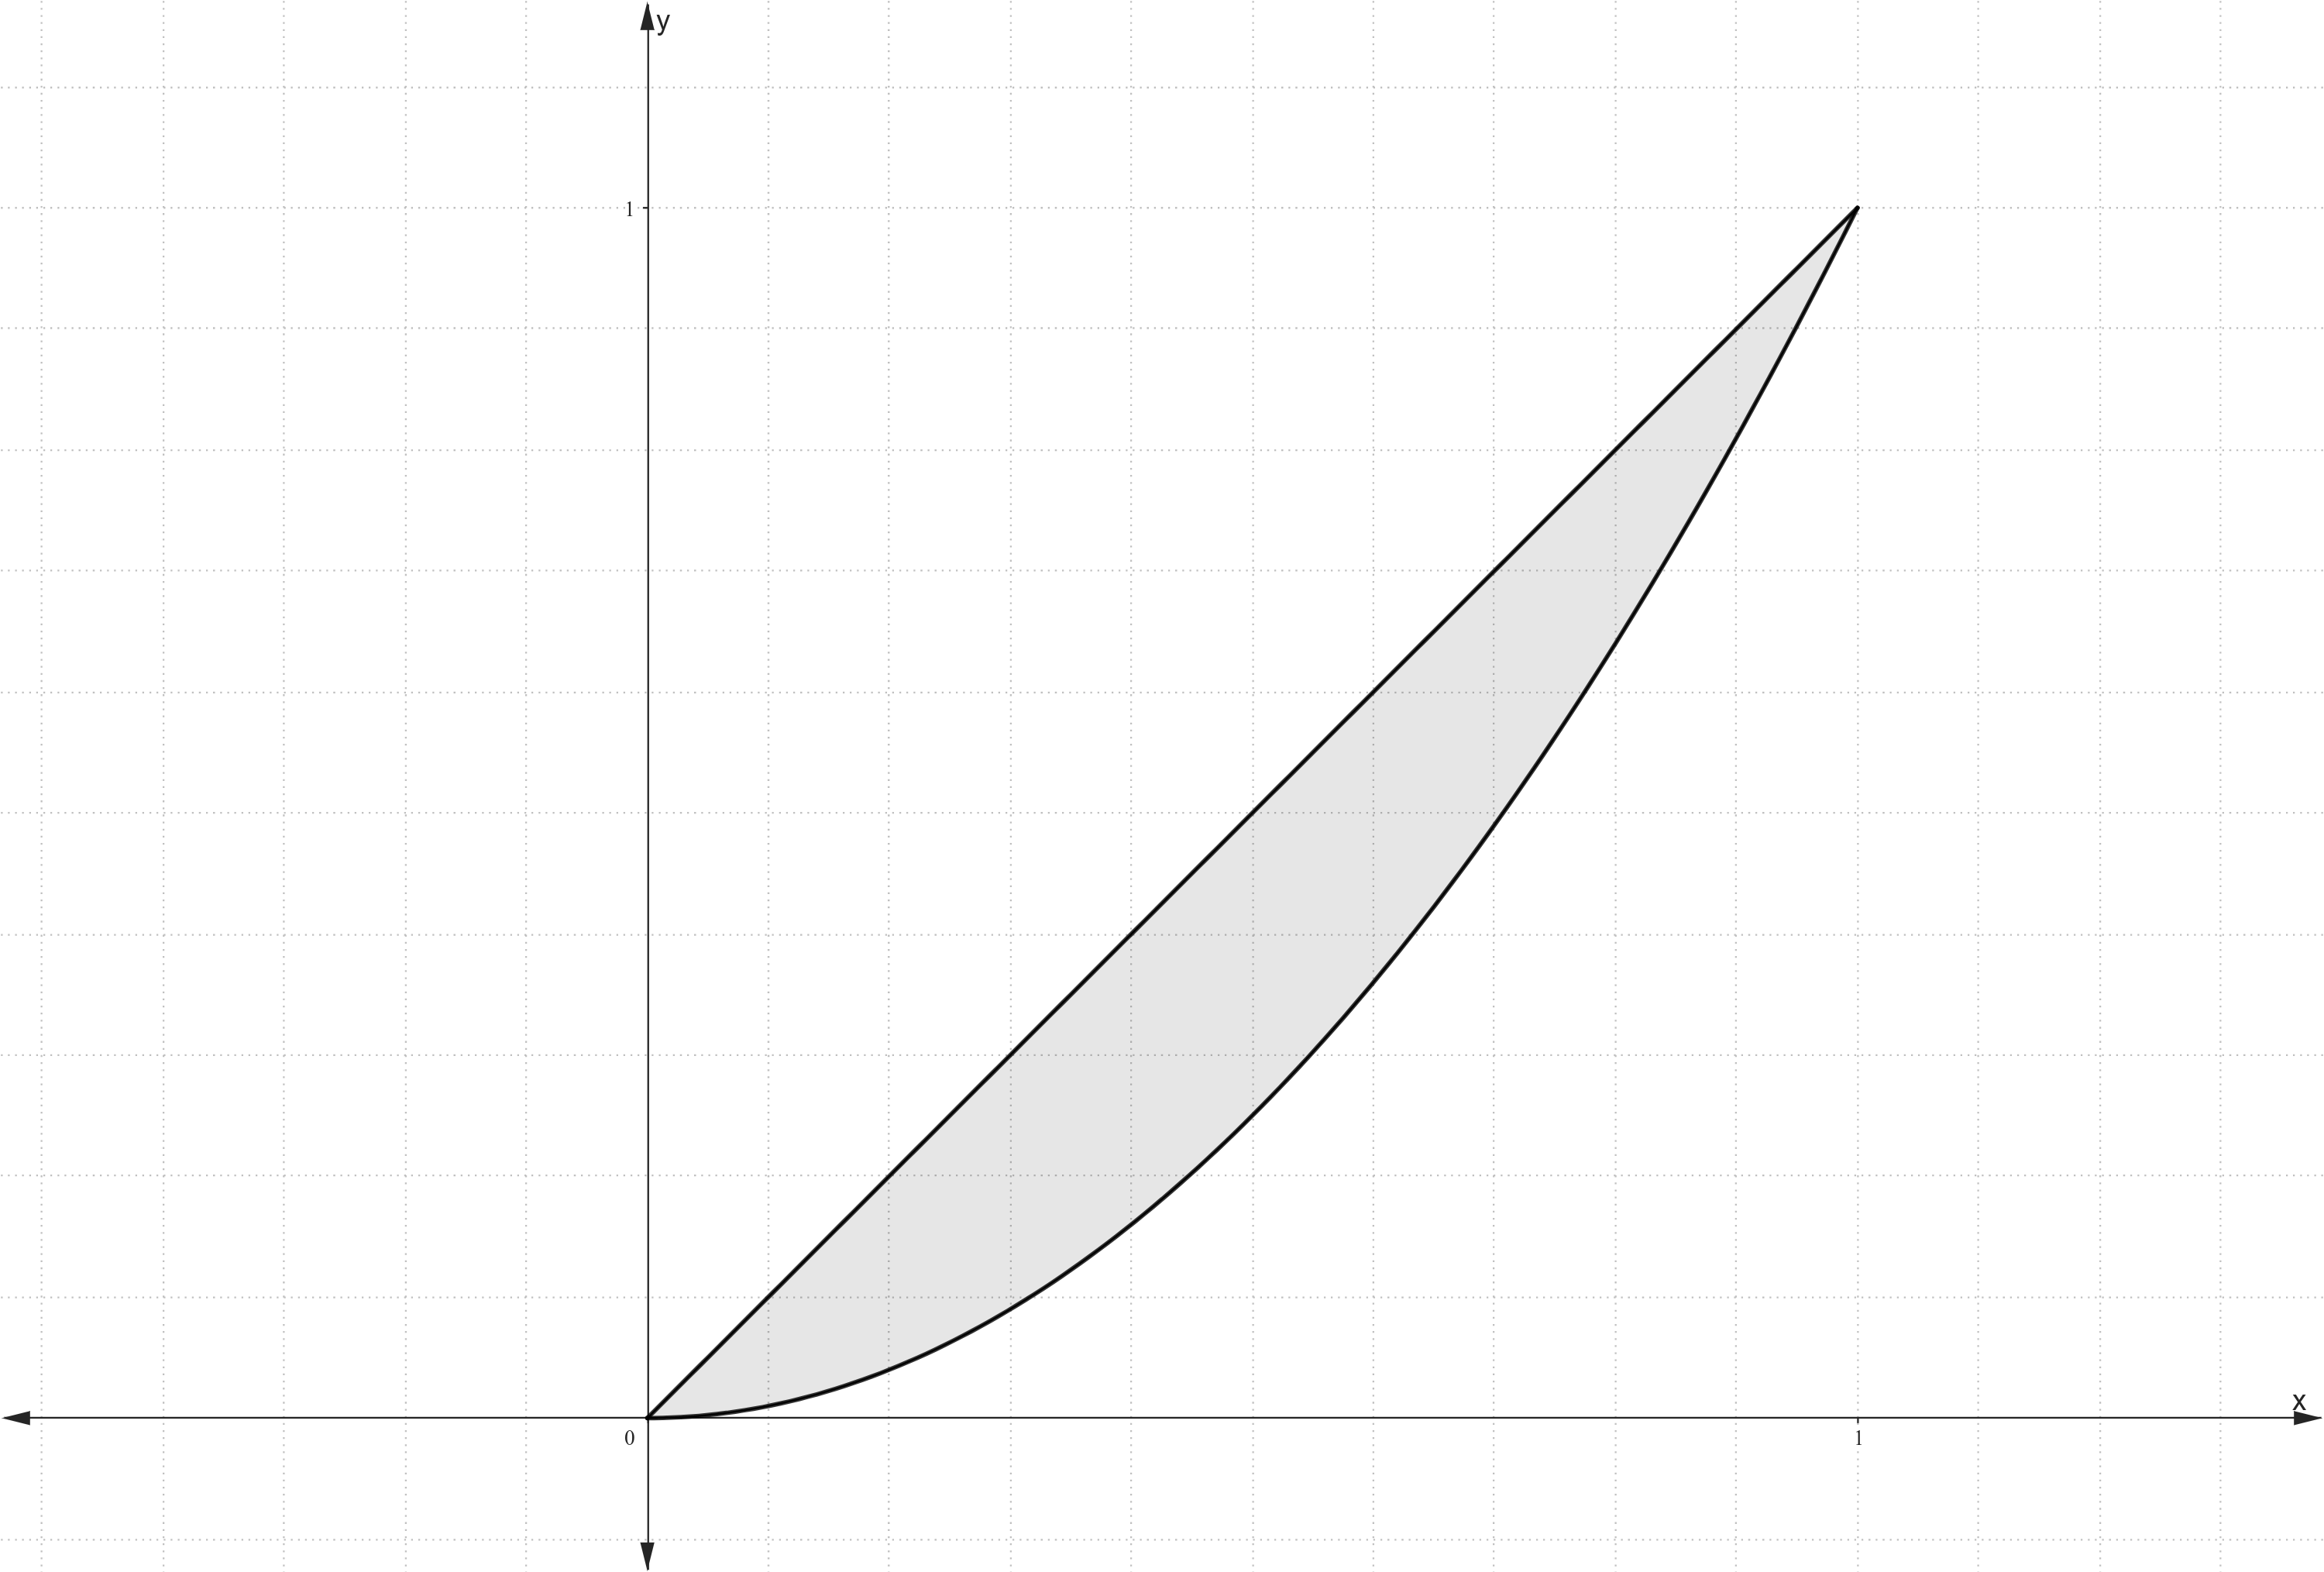
\includegraphics[width=0.5\textwidth]{../figures/simpleRegion.png}
        \caption{Plot of the region $H$.}
        \label{fig1:19}
    \end{figure}
\end{Eg}
\

\textbf{Exercise.} Show that the region bounded by $x^2 + y^2 \leq 1$ and $y \geq 0$ in $\R^2$ is both a $x$-simple as well as $y$-simple region.



\end{document}